\documentclass[11pt]{article}

%% LaTeX Preamble - Common packages

\usepackage[utf8]{inputenc}
\usepackage[spanish]{babel}
\usepackage{graphicx}
\usepackage{amsmath,amssymb}
\usepackage[left=2cm,right=2cm,top=2cm,bottom=2cm]{geometry}

\spanishdecimal{.}

\title{Examen rápido No. 6}
\author{Reconocimiento de Patrones (2023-2)}
\date{Julio Waissman Vilanova} % delete this line to display the current date

%%% BEGIN DOCUMENT
\begin{document}

\maketitle

\vspace{5mm}

\textbf{Nombre}: \line(1,0){400}

\vspace{9mm}


\begin{enumerate}



\item Considera la siguiente figura:

\begin{center}
  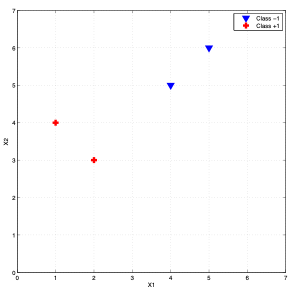
\includegraphics[width = 0.8\textwidth]{svm-1.png}
\end{center}

Dibuja el margen de fase y circula los vectores de soporte, si usamos un SVM lineal para clasificar los datos.


\item Uno de los kernels más utilizados es el kernel tipo RBF el cual está dado por:

$$
k(x^{(i)}, x^{(j)}) = \exp(- \frac{||x^{(i)} - x^{(j)}||^2}{2\sigma}).
$$

Supongamos que tenemos 3 puntos en el espacio, $x^{(i)}$, $x^{(j)}$ y $x$, donde $x$ es geométricamente cercano a $x^{(i)}$ y geométricamente lejano a $x^{(j)}$. Selecciona la respuesta correcta: 

\begin{itemize}
    \item $k(x^{(i)}, x)$ es cercano a 1 mientras que $k(x^{(j)}, x)$ es cercano a 0.
    \item $k(x^{(i)}, x)$ es cercano a 0 mientras que $k(x^{(j)}, x)$ es cercano a 1.
    \item $k(x^{(i)}, x) \gg 1$  mientras que $k(x^{(j)}, x) \ll 0$.
    \item $k(x^{(i)}, x) \ll 0$  mientras que $k(x^{(j)}, x) \gg 1$.
\end{itemize}


\item ¿Que son los vectores de soporte? Puede haber varias respuestas (o ninguna):
\begin{itemize}
    \item Los datos $x^{(i)}$ del conjunto de aprendizaje más lejanos a la frontera de decisión para un clasificador SVM.
    \item Los únicos datos $x^{(i)}$ del conjunto de aprendizaje necesarios para calcular $h^*(x)$ en un clasificador SVM.
    \item Los centroides de las clases.
    \item Todos los datos $x^{(i)}$ del conjunto de aprendizaje con $\alpha_i \neq 0$.
    \item Los datos $x^{(i)}$ del conjunto de aprendizaje tales que $(w^T x^{(i)} + b) y^{(i)} = 1$.
\end{itemize}


\item Se entrenó un clasificador tipo SVM con kernel polinomial ($p = 3$) sobre un conjunto de datos y se obtuvo un error en el conjunto de muestra por debajo del requerimiento establecido. Desafortunadamente, el error fuera de muestra en el conjunto de validación era muy grande. Selecciona las acciones que creas podrían mejorar nuestro clasificador:

\begin{itemize}
    \item Aumentar el valor de $C$
    \item Disminuir el valor de $C$
    \item Usar un kernel lineal
    \item Usar un kernel RBF
    \item Solicitar más datos
    \item Reducir el número de características utilizadas
    \item Generar nuevas características
    \item Usar el kernel polinomial pero con $p=2$
    \item Usar el kernel polinomial pero con $p=4$
    \item Usar \emph{k-fold cross validation}
    \item Rezar
\end{itemize}

\item ¿Un clasificador SVM lineal encuentra los mismos parámetros $w$ y $b$ que si usamos el método de regresión logística? ¿Pasa siempre? Si no ¿En que casos puede pasar? Justifica tus respuestas

\end{enumerate}
\end{document}